\section{The Reasoning Framework}
\label{sec:reasoning}

We now describe a proof system that lets us demonstrate that a \txnimp
program satisfies its high-level invariants in all small-step
executions that satisfy a chosen trace invariant\footnote{It is
important to mind the distinction between high-level invariants
(\eg~\C{X$\ge$0}) and trace invariants (\eg~\C{RC}). The former
constitute \emph{proof} \emph{obligations} for the programmer, whereas
the latter capture \emph{assumptions} about the machine. } ($\I$).
Since the trace invariant is a conjunction of store consistency
($\I_s$) and transaction isolation ($\I_c$) constraints, the
demonstration is a proof that the program preserves its invariants
when executed on a chosen store under a selection of isolation levels
for its transactions.

As mentioned earlier, our proof system is a rely-guarantee framework
that admits compositional reasoning by abstracting away the
environmental interference as a rely relation. A conspicuous
difference between a standard development of rely-guarantee and ours
is that, while the former reasons in terms of program states (variable
to value bindings), we reason in terms of executions as captured by
their traces ($\E$). In particular, our rely ($R$) and guarantee ($G$)
relations relate executions (i.e., $R,\,Q\,\subseteq\,\E\times\E$),
and pre ($P$) and post ($Q$) conditions are assertions over executions
(i.e., $P,\,Q\, : \E \rightarrow \Prop$). Our development nonetheless
facilitates state-based reasoning via the interpretation function
($\interp{\cdot}$) introduced in \S\ref{sec:syntax}. For example, if a
\emph{bi-state} rely relation relates every pair of states $\sigma$
and $\sigma'$ such that $\sigma'(X) \ge \sigma(X) \ge 0$, the
corresponding \emph{bi-execution} rely relation relates every pair of
executions $\E$ and $\E'$ such that $\interp{\E}(X) \ge
\interp{\E'}(X) \ge 0$.  Assertions on state are also written
similarly. For instance, consider the postcondition
$\C{C\,=\,k-a1-a2}$ of the program in Fig.~\ref{fig:motiv-eg-1}. The
corresponding assertion on the post-state
($\lambda\sigma.~\sigma(\C{C}) \,=\, \C{k-a1-a2}$) asserts that in all
states resulting from executing the program, the value of \C{C} is
\C{k-a1-a2}. The equivalent execution-based assertion
($\lambda\E.~\interp{\E}(\C{C})\,=\,\C{k-a1-a2}$) asserts that in all
executions of the program, the value of \C{C} is \C{k-a1-a2}.
However, having access to an execution facilitates assertions that go
beyond the state. An example is an invariant of \C{Wd1} described
abstractly in \S\ref{sec:motivation}, and reified as an
execution-based assertion below:
\begin{smathpar}
\begin{array}{l}
  \lambda\E.~ \neg(\underE{\committed(\C{Wd1}}) \conj 
      \underE{\C{Wd1} \wrstoar \C{C}}\\
  \hspace*{0.2in}\conj(\neg(\underE{\committed(\C{Wd2})}) \Rightarrow 
      \C{\interp{\E}(C) = k-a1}) \\
   \hspace*{0.2in}\conj (\underE{\committed(\C{Wd2})} \Rightarrow 
      \C{\interp{\E}(C) = k-a1-a2})
\end{array}
\end{smathpar}
% Where, $\committed$ is defined as:
% \begin{smathpar}
% \begin{array}{lcl}
% \underE{\committed(T_i)} & \Leftrightarrow &
%   \exists\eta.~\underE{\eta\in T_i} \conj \kind(\eta) = \C{COMMIT}\\
% \end{array}
% \end{smathpar}
One of the conjuncts asserts that \C{Wd1} has written to \C{C} - a
fact which cannot be deduced solely from the value of \C{C} (esp. in
presence of interference), but can be expressed as a proposition over
the execution trace.

\subsection{The Rely-Guarantee Judgment}
\label{sec:rely-guarantee}

\begin{figure}[t]
\raggedright
%
\fbox {\( \R \vdash \hoare{P}{c}{Q} \)} 
\quad \fbox {\( \rg{I,R}{c}{G,I} \)}\\[4pt]
%\fbox{\( \rg{\mathbb{I},P,R}{\txnbox{c}_i}{G,Q}\)} \quad
%\fbox{\( \rg{\mathbb{I},P,R}{c}{G,Q}\)} \quad\\
%
\begin{minipage}{3.1in}
\rulelabel{RG-Update}
\begin{smathpar}
\begin{array}{c}
\RULE
{
  \stable(\R,Q)\\
  \forall\stl,\stl',\stg.~P(\stl,\stg) \conj \\
  \stl' = \stl \cup \{r' \,|\, \exists(r\in\Delta).[r/x]e_2 \conj\\
  \hspace*{.7in} r'=[r/x]e_1\} \Rightarrow   Q(\stl',\stg)
}
{
  \R \vdash \hoare{P}{\updatee{\lambda x.e_1}{\lambda x.e_2}}{Q}
}
\end{array}
\end{smathpar}
\end{minipage}
%
%
\begin{minipage}{3in}
\rulelabel{RG-Select}
\begin{smathpar}
\begin{array}{c}
\RULE
{
  \\
  \R \vdash \hoare{P'}{c}{Q}\spc
  \stable(\R,P')\\
  P'(\stl,\stg) \Leftrightarrow P(\stl,\stg) \wedge
  x = \{r' \,|\, \exists(r\in\Delta).~ [r/y]e_2\} \\
}
{
  \R \vdash \hoare{P}{\lete{x}{\selecte{\lambda y.e}}{c}}{Q}
}
\end{array}
\end{smathpar}
\end{minipage}
%
\bigskip

%
\begin{minipage}{3.2in}
\rulelabel{RG-Delete}
\begin{smathpar}
\begin{array}{c}
\RULE
{
  \stable(\R,Q)\\
  \forall\stl,\stl',\stg.~P(\stl,\stg) \conj 
  \stl' = \stl \cup \{r' \,|\, \exists(r\in\Delta).~ [r/x]e
        \conj r'=\{\bar{f}=r.\bar{f}; \idf=r.\idf;
        \delf=\C{true}\}\}
  \Rightarrow 
  Q(\stl',\stg)
}
{
  \R \vdash \hoare{P}{\deletee{\lambda x.e}}{Q}
}
\end{array}
\end{smathpar}
\end{minipage}
%
\bigskip

%
\begin{minipage}{3.2in}
\rulelabel{RG-Insert}
\begin{smathpar}
\begin{array}{c}
\RULE
{
  \stable(\R,Q)\\
  \hspace*{-1.1in}\forall\stl,\stl',\stg,i.~P(\stl,\stg) \conj i \not\in
  \dom(\stl\cup\stg) \\
  \conj \stl'=\stl \cup 
  \{\{\bar{f}=x.\bar{f};\,\idf=i;\,\delf=\C{false}\} \Rightarrow 
  Q(\stl',\stg)
}
{
  \R \vdash \hoare{P}{\inserte{x}}{Q}
}
\end{array}
\end{smathpar}
\end{minipage}
%
%
\begin{minipage}{3in}
\rulelabel{RG-Foreach}
\begin{smathpar}
\begin{array}{c}
\RULE
{
  \stable(\R,Q)\spc
  \stable(\R,\psi)\\
  P \wedge y=\emptyset \Rightarrow \psi\spc
  \R \vdash \hoare{\psi \wedge z\in x}{c}{Q_c}\\
  Q_c \wedge z\in y \Rightarrow \psi\spc
  \psi \wedge y=x \Rightarrow Q
}
{
  \R \vdash \hoare{P}{\foreache{x}{\lambda y.\lambda z.c}}{Q}
}
\end{array}
\end{smathpar}
\end{minipage}
%
\bigskip

%
\begin{minipage}{3.9in}
\rulelabel{RG-Txn}
\begin{smathpar}
\begin{array}{c}
\RULE
{
  \stable(R,\I)\spc
  P(\stl,\stg) \Leftrightarrow \stl=\emptyset \wedge I(\stg)\\
  \R_l(\stl,\stg,\stg') \Leftrightarrow \exists \stg_1. \I_e(\stl, \stg_1, \stg) \wedge R(\stg, \stg') \wedge \I_e(\stl, \stg_1, \stg')\\
  \R_c(\stl,\stg,\stg') \Leftrightarrow \exists \stg_1. \I_c(\stl, \stg_1, \stg) \wedge R(\stg, \stg') \wedge \I_c(\stl, \stg_1, \stg')\\
  \R_l \vdash \rg{P}{c}{Q} \spc \stable(\R_c,Q)\\
  \forall \stl,\stg.~ Q(\stl,\stg) \Rightarrow 
    G(\stg, \stl \gg \stg)\spc
  \forall \stg,\stg'.~I(\stg) \wedge G(\stg,\stg') \Rightarrow I(\stg')\\
}
{
  \rg{I,R}{\ctxn{i}{\I}{c}}{G,I}
}
\end{array}
\end{smathpar}
\end{minipage}
%
%
\begin{minipage}{2in}
\rulelabel{RG-Conseq}
\begin{smathpar}
\begin{array}{c}
\RULE
{
  \rg{I,R}{\ctxn{i}{\I}{c}}{G,I}\\
  \I' \Rightarrow \I \spc 
  R' \subseteq R \\
  \stable(R',\I')\spc
  G \subseteq G' \\
  \forall \stg,\stg'.~I(\stg) \wedge G'(\stg,\stg') \Rightarrow I(\stg')\\
}
{
  \rg{I,R'}{\ctxn{i}{\I'}{c}}{G',I}
}
\end{array}
\end{smathpar}
\end{minipage}
%

\caption{\small \txnimp: Rely-Guarantee Rules}
\label{fig:rg-rules}
\vspace*{-12pt}
\end{figure}


The standard rely guarantee judgment is the quintuple
$\rg{P,R}{c}{G,Q}$, which intuitively means the following: if a
command $c$ is executed in a state that satisfies its precondition
$P$, provided that every interference step during the execution is
contained inside the rely relation $R$, then the effect that each step
of executing $c$ has on the state is captured by $G$, and the final
state of execution satisfies the postcondition $Q$. The terms
``execution'' and ``step'' are defined with respect to an operational
semantics, which, in our case, is parameterized on the trace invariant
$\I$. Consequently, our rely-guarantee judgment for commands is the
sextuple $\rg{\I,P,R}{c}{G,Q}$, whose semantics differs from the
quintuple in that it requires every step of the execution to preserve
the trace invariant $\I$ for the postcondition to be valid.  As usual,
if $c$ is inside a transaction $T_i$, we write $\txnbox{c}_i$. \txnimp
expressions are side-effecting (they generate \C{RD} effects), and
admit interference during their evaluation.  Therefore, like the
commands, expressions need to be reasoned about explicitly. But,
unlike commands, expressions evaluate to values, and the reasoning
framework should also admit assertions on such values.  We therefore
define a separate judgment for expressions - the septuple
$\rg{\I,P,R}{e}{G,C,Q}$. The new entrant $C : \mathbb{N} \rightarrow
\Prop$ is an assertion on the return value of $e$.

The rules that define rely-guarantee judgment are shown in
Fig.~\ref{fig:rg-rules}. Like the standard definitions of rely
guarantee, our definition also relies on the \emph{stability}
condition, which requires pre and post conditions to hold despite the
interference from concurrent threads (captured by $R$). The stability
of pre and post conditions can be predicated on the assumption that
the interference preserves the trace invariant $\I$. Formally:
\begin{smathpar}
\begin{array}{lcl}
  \underI{\stable(R,P)} & \defeq & \forall \E, \E'.\, 
  \I(\E) \conj P(\E) \conj R(\E,\E') \\
  &   & \hspace*{1in}\conj \I(\E') \Rightarrow P(\E')\\
\end{array}
\end{smathpar}
However, the assumption that the interference preserves $\I$ (or,
dually, $\I$ withstands inteferference) needs to be justified
separately. We call this the stability requirement on $\I$:
\begin{smathpar}
\begin{array}{lcl}
\stable(R,\I)& \defeq & \forall \E, \E'.\, 
  \I(\E) \conj R(\E,\E')\Rightarrow \I(\E')\\
\end{array}
\end{smathpar}

The rule \rulelabel{RG-Var} defines the rely-guarantee judgment for
shared variable reads inside a transaction $T_i$. It requires $\I$ to
be stable, and pre and post conditions to be stable relative to $\I$.
The quantified premise effectively requires a proof that if the
abstract machine of Fig.~\ref{fig:txnimp} takes a step starting from
an execution $\E$ that satisfies the precondition $P$, then the
resultant execution $\E'$ satisfies the postcondition $Q$, and that
the guarantee $G$ faithfully captures the transition from $\E$ to
$\E'$. It is informative to compare this premise with the premise of
the \rulelabel{E-Aux} reduction rule of Fig.~\ref{fig:txnimp}. Similar
premises also appear in \rulelabel{RG-Asgn} and \rulelabel{RG-Txn}
rules, which define rely-guarantee judgments for assignments and
transactions, respectively. \rulelabel{RG-Var} however also requires
the return value ($\interp{S}(X)$) of the read to satisfy the
assertion $C$ meant for the value. \rulelabel{RG-Arith} defines the
RG judgment for an arithmetic expression $e_1\pm e_2$ in terms of the
corresponding judgments for the constitutent expressions $e_1$ and
$e_2$. The quantified premise requires any value resulting from
evaluating $e_1 \pm e_2$ to satisfy the assertion $C$, provided that
$e_1$ and $e_2$ always evaluate to values that satisfy $C_1$ and
$C_2$, respectively. The rules for sequential and parallel composition
of comands are more-or-less same as the corresponding rules in
classical rely-guarantee, hence elided.

% RG judgment for the assignment $X:=e$ makes use of the corresponding
% judgment for the RHS expression $e$. The quantified premise asserts
% that evaluating the assigment after evaluating $e$ to a value $v$ and
% an execution $\E$, should result in an execution $\E'$ that satisfies
% the postcondition $Q$, while being related to $\E$ via the guarantee
% $G$. RG judgment for the \C{txn} lexical block is similar.  It uses
% the judgment for the transaction-bound command $c$ (i.e.,
% $\txnbox{c}_i$) to obtain an invariant $Q'$ for the execution $\E$
% before the commit, and verifies that committing the transaction under
% $\E$ results in an execution $\E'$ that satisfies transaction's
% postcondition $Q$. As usual, $\E$ and $\E'$ need to be related by $G$.
% The rules for sequential composition of transaction-bound comands
% (\rulelabel{RG-Seq}) and parallel composition of top-level commands
% (\rulelabel{RG-Par}) are straightforward, and more-or-less same as the
% corresponding rules in classical rely-guarantee.

The \rulelabel{RG-Conseq} rule defines ways to strengthen or weaken
relations and assertions associated with the RG judgment of
transaction-bound expressions. Similar rules exist for
transaction-bound and top-level commands, but are not shown. In
particular, the rules allow the precondition $P$ and the rely relation
$R$ to be strengthened\footnote{A stronger relation is a smaller set
than a weaker relation, hence a stronger $R$ admits lesser
interference than a weaker $R$}, and the postcondition $Q$ (also, $C$
in the case of expressions) and the guarantee relation $G$ to be
weakened. This kind of strengthening/weakening is also admitted in the
classical RG framework. The most notable aspect of
\rulelabel{RG-Conseq} rules however is that they allow the trace
invariant $\I$ to be strengthened. Considering that $\I$ captures
isolation properties, this means that a program proved correct under
weaker isolation levels is also correct under stronger levels.
Parametricity over the trace invariant $\I$, combined with the ability
to strengthen $\I$ as needed, allows our proof system to admit a
highly flexible proof strategy to prove programs correct on various
stores. For example, programmers can \emph{define} isolation
guarantees of their choice (by defining $\I$ appropriately) and then
prove programs correct assuming the guarantees hold. Soundness of
strengthening $\I$ assures that the program can now be executed safely
on any real store that offers same or stronger isolation guarantees
than those assumed. The following subsection proves the soundness of
our proof system.

\subsection{Semantics and Soundness}

We now formalize the semantics of the rely-guarantee judgment of
Fig.~\ref{fig:rg-rules} through a series of definitions.

\begin{definition}[Step-indexed reflexive transitive closure]
Forall $A$, $R: A \rightarrow A \rightarrow \mathbb{P}$, and $n :
\mathbb{N}$, step-indexed reflexive transitive closure $R^n$ of $R$ is
the smallest relation satisfying the following
properties:
\begin{itemize}
\item $\forall (x:A).\, R^0 (x,x)$
\item $\forall (n:\mathbb{N})(x,y,z : A).\, R(x,y) \conj R^n(y,z) \Rightarrow
R^{n+1}(x,z)$
\end{itemize}
\end{definition}

\begin{definition}[Interleaved step and multi-step relations]
Interleaved step relation interleaves the thread-local reduction with
the interference from concurrent threads captured as the rely relation
($R$).  It is defined as following:
\begin{smathpar}
\begin{array}{lcl}
\I \vdash (c,\E) \rstepsto (c',\E') & \defeq & \I \vdash 
  (c,\E) \stepsto (c',\E') \\
  &   & \disj (c' = c \conj R(\E, \E') \conj \I(\E'))\\
\end{array}
\end{smathpar}
The interleaved step relation for transaction bound expressions
($\txnbox{e}_i$) and commands ($\txnbox{c}_i$) is defined similarly.
Interleaved multi-step relation ($\stepssto{n}$) is the step-indexed
reflexive transitive closure of the interleaved step relation.
\end{definition}

\begin{definition}[Semantics of the RG judgment]
Semantics of the RG sextuple $\rg{\mathbb{I},P,R}{c}{G,Q}$ is defined
in terms of the interleaved step relation as following:
\begin{smathpar}
\begin{array}{l}
\hspace*{-0.3in}
\rg{\mathbb{I},P,R}{c}{G,Q} \;\defeq\; \forall \E.\, P(\E)
  \wedge \mathbb{I}(\E) \\
\hspace*{0.4in}\Rightarrow (\forall n,\E'.\; \I \vdash (c,\E) 
    \rstepssto{n} (\cskip,\E') \Rightarrow Q(\E')) \\
\hspace*{0.5in}\conj \texttt{step-guaranteed}(\I,R,G,c,\E)\\
\end{array}
\end{smathpar}
The first conjunct in the consequent is called the \emph{Hoare
consequent} since it ascribes Hoare triple semantics to RG sextuple.
The second conjunct, called the \emph{guarantee consequent}, uses the
$\texttt{step-guaranteed}$ predicate defined below:
\begin{smathpar}
\begin{array}{l}
\texttt{step-guaranteed}(\I,R,G,c,\E) \;\defeq\; \forall n,\E',c'',\E''.\\
\hspace*{0.2in}\I \vdash (c,\E) \rstepssto{n} (c',\E') \conj \I \vdash (c',\E') \stepsto
  (c'',\E'') \Rightarrow G(\E',\E'')\\
\end{array}
\end{smathpar}
The guarantee consequent requires $G$ to capture the trace effect of
every small-step of $c$, where the reduction can be interleaved by the
interference ($R$) from concurrent threads. Semantics of the RG
sextuple for transaction-bound commands ($\txnbox{c}_i$) is defined
similarly. Expressions, unlike commands, evaluate to a value $v$, and
the semantics of their RG septuple
($\rg{\I,P,R}{\txnbox{e}_i}{G,C,Q}$) differs slightly in that its
Hoare consequent requires the value $v$ to satisfy the assertion $C$. 
\end{definition}

It is worthwhile to note that the semantics of all RG judgments,
including the judgments for transaction-bound terms,  make similar
demands of the guarantee relation. Considering that transactions are
atomic (though not isolated), at a first glance, it might seem odd
that a transaction's guarantee is required to make explicit every step
of its reduction. This requirement is however justifed because, in
reality, a transaction's atomicity is predicated on the isolation
settings of the observer. A \iso{Read Uncommitted} transaction, for
example, can observe the internal state of a transaction, regardless
of the latter's preferences\footnote{Thus, there is no such thing as
atomicity; it's all about isolation.}. In the interest of modular
verification, the transaction must therefore make its internal state
available via its guarantee relation.

Soundness of rely-guarantee judgments can now be stated
thus\footnote{Supplementary contains a rigorous proof of the soundness
theorem, and all relevant lemmas.}:
\begin{theorem}[Soundness] 
Rely-guarantee judgments defined by the rules in
Fig.~\ref{fig:rg-rules} are sound with respect to their semantics
defined above. 
\end{theorem}
\noindent In particular, if $\rg{\I,P,R}{c}{G,Q}$ can be derived using
the rules of Fig.~\ref{fig:rg-rules}, then (a). every interleaved
multi-step reduction of $c$ starting from a trace that satisfies $P$
and $\I$, results in a trace that satisfies $Q$, and (b). the effect
that every small-step of $c$ has on the trace is contained in $G$.
Soundness of RG judgment for transaction-bound commands
($\txnbox{c}_i$) is stated similarly.  For expressions, soundness of
the judgment $\rg{\I,P,R}{\txnbox{e}_i}{G,C,Q}$ also proves that $e$
is always evaluated to a value that satisfies $C$.

\subsection{Soundness under Eventually Consistent Replication}

\begin{figure}
\centering
\subcaptionbox {
  Replica model
  \label{fig:ec-theirs}
} [
  0.4\columnwidth
] {
  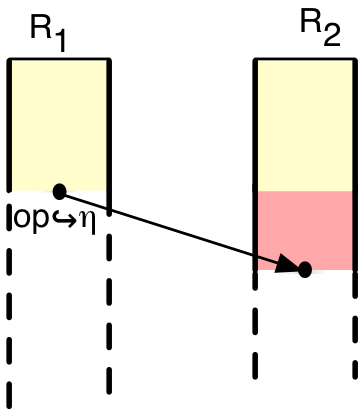
\includegraphics[scale=0.7]{Figures/ec-theirs}
 
}
\hspace*{0.1in}
\subcaptionbox {
  Subset model
  \label{fig:ec-ours}
}{
  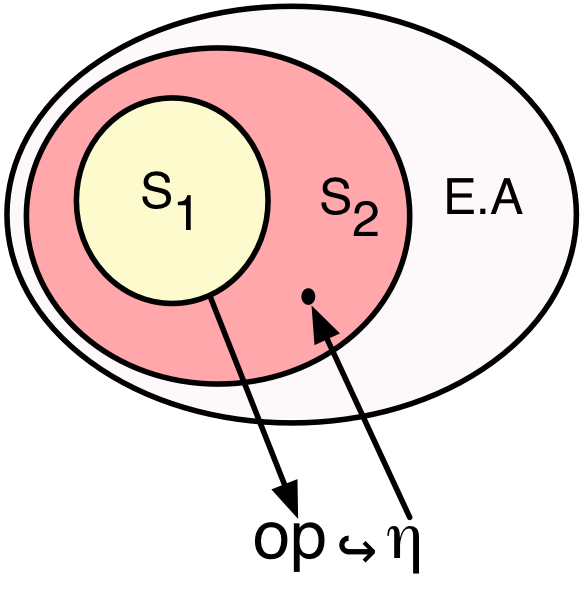
\includegraphics[scale=0.45]{Figures/ec-ours}
} \caption{In the replica model, operation $\op$ generates effect
$\eta$ at replica $R_1$, which is then merged to $R_2$. If the
\emph{store is {\sc cc}}, then $R_2$'s state at merge event is same or
larger than $R_1$'s state at generation event (the difference is
highlighted). In our subset model, $\op$ witnesses $S_1 \subseteq
\E.\A$ and generates $\eta$, which is immediately added to $\E.\A$. A
later operation may witness $S_2 \subseteq \E.\A$, and if the
\emph{operation is} {\sc cc} and $\eta \in S_2$, then it also
witnesses $S_1$ (i.e., $S_1 \subseteq S_2$). } 
% Moreover, Like $R_2 - R_1$, if all effects in $S_2 - S_1$ are
% concurrent with $\eta$, i.e., $\not\exists\eta'.~\eta' \in S_2 - S_1
% \conj % visZ(\eta,\eta')$, then any precondition $P$ that is valid
% when $\op$ executed is also valid when $\eta$ is witnessed because
% of the stability condition.
\label{fig:ec-theirs-vs-ours}
\end{figure}

In this section, we present an intuitive explanation of the soundness
result in context of eventually consistent replication. 
% In other words, we explain why our approach is a sound way of
% reasoning about transactions under eventually consistent replication
% despite our system model not including the standard artifacts
% associated with a replicated store. 


Existing approaches to reason about eventually consistent replication
necessarily involve reasoning in terms of \emph{replicas} of data. The
primary challenge in this setting is to ensure that the assumptions
made and guarantees enforced by an operation at one replica carry over
to other replicas that merge its effects, thus preserving the overall
integrity of the system. Reasoning frameworks, such
as~\cite{gotsmanpopl16}, address this challenge by imposing
restrictions on how various replica states differ, i.e., by
strengthening the consistency of the store. Our view of eventually
consistent replication however does not explicitly involve replicas.
Fig.~\ref{fig:ec-theirs-vs-ours} contrasts our model of EC replication
with the conventional replica-based model.  Under our model, the
notion of a replica is subsumed by the concept of visibility; a
replica is defined by the subset ($S$) of global state ($\E.\A$) that
an operation witnesses.  Constraints over replica states therefore
manifest as constraints over the visibility relation. For example,
instead of requiring the store to be causally consistent, an operation
can request to witness a causally consistent subset of the state; such
demands can be made via the trace invariant $\I$. For a precondition
($P$) of the operation to be useful, it has to be an assertion over
every causally consistent subset of the global state. Since any
replica that eventually executes the operation has to expose one such
subset ($S$), the precondition is guaranteed to hold regardless of the
replica. There is however one problem with this explanation; by
considering subsets of just one global state, it ignores the fact that
the global state (hence, the replica states) change during the
execution of the operation. Existing approaches account for this
change by distinguishing between \emph{effect generation} event at one
replica and \emph{effect merge} event at another replica, and
requiring that certain invariants be preserved between these two
events at different replicas. Our framework folds all of this into a
stability condition (\S\ref{sec:rely-guarantee}). Since any change to
the global state during the execution of the operation is an
interference, and $P$ is required to be stable with respect to any
such interference, it follows that $P$ is valid on every replica, thus
ensuring that assumptions made at the generation event are also valid
at the merge event.

\subsection{Examples}

\GK{Here, I plan to include the full example that we dropped from
\S\ref{sec:motivation}.}
